\begin{frame}{Fila de prioridade}
    \metroset{block=fill}

    \begin{block}{Definição}
        Uma {\bf fila de prioridade} é uma estrutura onde a remoção remove o elemento com maior valor.
    \end{block}

    A implementação da fila de prioridade é feita a partir de uma heap de máximo (cf. Cormen, Cap. 6). Por exemplo, uma heap de máximo armazenando os elementos $\{1, 2, 3, 4, 7, 8, 9, 10, 14, 16\}$ é

    \begin{figure}
        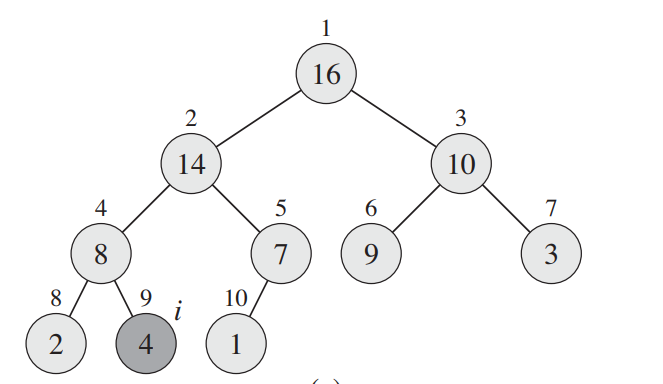
\includegraphics[scale=0.25]{max-heap.png}
    \end{figure}
    
\end{frame}

